\documentclass[12pt,a4paper]{article}
\usepackage{geometry}
\usepackage{slashbox}
\geometry{
	a4paper,
	total={170mm,257mm},
	left=20mm,
	right=20mm,
	top=20mm,
	bottom=20mm
}
\usepackage{graphicx}
\usepackage{pdfpages}
\usepackage{placeins}
\usepackage{float}

\usepackage{polski}
\usepackage[utf8]{inputenc}

\begin{document}
	
	\begin{titlepage}
		\newgeometry{top=5.5cm, bottom=3cm}
		
		\centering
		{\huge\bfseries Logika układów cyfrowych lab.\par}
		
		\vspace{0.5cm}
		Prowadzący: Mgr inż. Antoni Sterna (E02-38m, wtorek 17:05) \\
	
		\vspace{1.1cm}
		{\Large sprawozdanie 8 - 2017.12.04\par}
		\vfill
		
		{\large\bfseries Jakub Dorda 235013\par}
		{\large\bfseries Marcin Kotas 235098\par}
		
		\vspace{1cm}
		\today \\ \LaTeX
		
		\restoregeometry
	\end{titlepage}

	\newgeometry{top=1.5cm, bottom=1.5cm, left=20mm, right=20mm}

	\section{Wprowadzenie/cel ćwiczeń}
	
		Celem ćwiczeń było zaprojektowanie analizatora ciągu par w czasie trwania zajęć. Dodatkowo należało przeprowadzić syntezę strukturalną  w wariancie Mealy z wykorzystaniem przerzutników JK w celu uruchomienia go na zestawie UNILOG.
		
	\section{Tabela prawdy i tablice Karnaugh:}
		
		\subsection{Minimalizacje:}
	
		\subsection{Użyte wzory:}
		
		\subsection{Schemat układu:}
		
		\vspace{1.5cm}
		\begin{center}
			%\makebox[\textwidth]{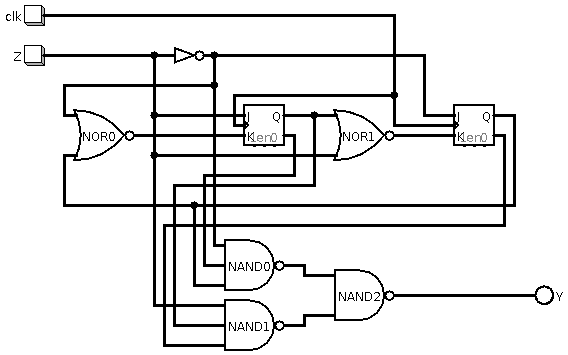
\includegraphics[width=\paperwidth - 40mm]{schem/circuit1.png}}
			Schemat 1 - analizator ciągu par w wersji Mealy
		\end{center}

	\section{Wnioski/podsumowanie}
	
			W celu sprawdzenia poprawności działania komparatora należało przeprowadzić testy dla wszystkich możliwych kombinacji wejść oraz stanów. W czasie testowania układu okazało się, że typ zbocza sygnału reset może mieć
			wpływ na poprawne zachowanie automatów ze względu na budowę wewnętrzną przerzutników. 
	
\end{document}